\documentclass{beamer}
\usepackage{ragged2e}
\usepackage{amsmath}
\usepackage{amsfonts}
\usepackage{amsthm}
\usepackage{mathrsfs}
\usepackage{CJKutf8}
\usepackage{tikz}
\setbeamertemplate{theorems}[numbered]
\justifying\let\raggedright\justifying
\begin{document}
\begin{CJK*}{UTF8}{gbsn}


  
\theoremstyle{definition}
\newtheorem{Def}{定义}
\theoremstyle{example}
\newtheorem*{Ex}{例:}
\newtheorem*{Thm}{定理}
\newtheorem*{Exercise}{习题}

\date{}
\author{陈建文}
\title{集合论与图论基本概念}
\begin{frame}
  \titlepage
\end{frame}

\begin{frame}
  \begin{Def}
通常把一些互不相同的东西放在一起所形成的整体叫做一个集合。构成集合的每个东西叫做集合的元素。
给定一个集合$A$和一个元素$a$,用$a \in A$表示$a$是$A$的一个元素,用$a \notin A$表示$a$不是$A$的一个元素。
\end{Def}
\begin{Ex}
  \begin{itemize}
  \item $1\in \{1,2,3\}$
  \item $0\notin \{1,2,3\}$
  \end{itemize}
\end{Ex}
\end{frame}
\begin{frame}
\begin{Def}
设$A$,$B$为两个集合,如果$A$中的每个元素都是$B$中的元素,则称$A$为$B$的子集,记为$A \subseteq B$; 如果$A \subseteq B$且存在$x\in B$使得$x \notin A$,则称$A$为$B$的真子集,记为$A\subset B$。    
\end{Def}
\begin{Ex}
\begin{itemize}
  \item   $\{1,2,4\} \subseteq \{1,2,3,4,5\}$
\item $\{1,2,4\} \subset \{1,2,3,4,5\}$
\end{itemize}
\end{Ex}
\end{frame}

\begin{frame}
\begin{Def}
设$A$,$B$为两个集合,如果$A \subseteq B$且$B \subseteq A$,则称$A$与$B$相等,并记为$A=B$。
\end{Def}
\begin{Ex}
\begin{itemize}
\item   $\{1,2,3,4,5\} = \{3,4,2,1,5\}$
\item $\{x \in \mathcal{R} | x^2 -5x + 6 = 0\} = \{2,3\}$
\end{itemize}
\end{Ex}
\end{frame}




\begin{frame}
  \begin{Def}
  集合$S$的所有子集构成的集合称为$S$的幂集,记为$2^S$或者$\mathcal{P}(S)$。
\end{Def}
\begin{Ex}
  \begin{itemize}
  \item       $2^{\phi}=\{\phi\}$
\item     $2^{\{1\}}=\{\phi, \{1\}\}$
\item   $2^{\{1,2\}}=\{\phi, \{1\},\{2\},\{1,2\}\}$
\item   $2^{\{1,2,3\}}=\{\phi, \{1\},\{2\},\{1,2\},\{3\},\{1,3\},\{2,3\},\{1,2,3\}\}$
  \end{itemize}
\end{Ex}

  \end{frame}

  
  \begin{frame}
    \begin{minipage}{0.70\linewidth}
  \begin{Def}
    设$A,B$为任意的两个集合,至少属于集合 $A$ 与集合$B$之一的那些元素构成的集合称为$A$与$B$的并集,记为$A \cup B$。
  \begin{equation*}
      A\cup B = \{x|x \in A \lor x \in B\} 
    \end{equation*}
    (这里$\lor$表示“或者”)
  \end{Def}
\end{minipage}
\begin{minipage}{0.29\linewidth}
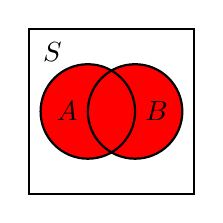
\begin{tikzpicture}[thick, scale=0.3]
  \draw (-3.5, -3.5) rectangle (3.5, 3.5);
  \filldraw[fill=red] (-1,0) circle [radius=2cm]
               (1,0) circle [radius=2cm];
  \draw (-1,0) node[left] {$A$};
  \draw (1,0) node[right] {$B$};
  \draw (-2.5,2.5) node {$S$};
\end{tikzpicture}
 \end{minipage}
 \begin{Ex}
   \begin{itemize}
   \item   $\{1,2\} \cup \{2,3\} = \{1,2,3\}$
   \end{itemize}
\end{Ex}
  \end{frame}

\begin{frame}
\begin{minipage}{0.70\linewidth}
  \begin{Def}
    设$A,B$为任意的两个集合,由既属于集合 $A$ 又属于集合$B$的所有元素构成的集合称为$A$与$B$的交集,记为$A \cap B$。
    \begin{equation*}
      A\cap B = \{x|x \in A \land x \in B\}
    \end{equation*}
  \end{Def}
\end{minipage}
\begin{minipage}{0.29\linewidth}
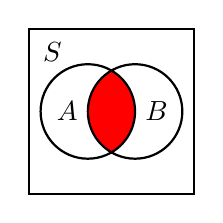
\begin{tikzpicture}[thick, scale=0.3]
  \draw (-3.5, -3.5) rectangle (3.5, 3.5);
  \fill[red] (-0.01, 0 |- -60:2cm) arc [start angle=-60, end angle = 60, radius = 2cm];
  \fill[red] (0.01, 0 |- 120:2cm) arc [start angle=120, end angle = 240, radius = 2cm];
  \draw (-1,0) circle [radius=2cm]
               (1,0) circle [radius=2cm];
  \draw (-1,0) node[left] {$A$};
  \draw (1,0) node[right] {$B$};
  \draw (-2.5,2.5) node {$S$};
\end{tikzpicture}
  \end{minipage}
  \begin{Ex}
    \begin{itemize}
    \item  $\{1,2\} \cap \{2,3\} = \{2\}$
    \end{itemize}
    \end{Ex}    
  \end{frame}
  \begin{frame}
     \begin{minipage}{0.70\linewidth}
  \begin{Def}
    设$A,B$为任意的两个集合,由属于集合$A$但不属于集合$B$的所有元素构成的集合称为$A$与$B$的差集,记为$A \setminus B$。
    \begin{equation*}
      A\setminus B = \{x|x \in A \land x \notin B\}
    \end{equation*}
  \end{Def}
\end{minipage}
\begin{minipage}{0.29\linewidth}
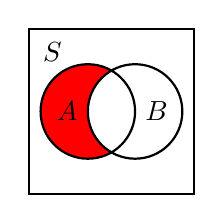
\begin{tikzpicture}[thick, scale=0.3]
  \draw (-3.5, -3.5) rectangle (3.5, 3.5);
\fill[red] (0,0 |- 60:2cm) arc [start angle=60, end angle = 300, radius = 2cm]
                           arc [start angle=240, end angle = 120, radius = 2cm];
  \draw (-1,0) circle [radius=2cm]
               (1,0) circle [radius=2cm];
  \draw (-1,0) node[left] {$A$};
  \draw (1,0) node[right] {$B$};
  \draw (-2.5,2.5) node {$S$};
\end{tikzpicture}
  \end{minipage}
  \begin{Ex}
    \begin{itemize}
    \item $\{1,2\} \setminus \{2,3\} = \{1\}$ 
    \end{itemize}
\end{Ex}
\end{frame}

\begin{frame}
  \begin{minipage}{0.70\linewidth}
  \begin{Def}
    在许多实际问题中,常以某个集合$S$为出发点,而所涉及的集合都是$S$的子集。这个包含所考虑的所有集合的集合$S$,称为该问题的全集。如果$A$为$S$的子集,则差集$S \setminus A$称为集合$A$对集合$S$的{\bfseries 补集},记为$A^c$。
    \begin{equation*}
      A^c = \{x|x \in S \land x \notin A\}
    \end{equation*}
  \end{Def}
\end{minipage}
\begin{minipage}{0.29\linewidth}
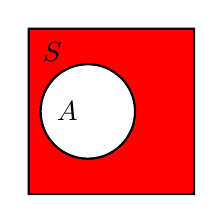
\begin{tikzpicture}[thick, scale=0.3]
  \filldraw[fill=red] (-3.5, -3.5) rectangle (3.5, 3.5)
               (-1, 0) circle [radius = 2cm];
  \draw (-1,0) node[left] {$A$};
  \draw (-2.5,2.5) node {$S$};
\end{tikzpicture}
\end{minipage}
\begin{Ex}
  \begin{itemize}
  \item $S = \{0,1\}, A =  \{0\},$ 则$A^c = \{1\}$。
  \end{itemize}
\end{Ex}
\end{frame}
\begin{frame}
  \begin{minipage}{0.69\linewidth}
  \begin{Def}
    设$A,B$为任意的两个集合,$A\setminus B$与$B\setminus A$的并集称为$A$与$B$的{\bfseries 对称差},记为$A \bigtriangleup B$。
    \begin{equation*}
      A\bigtriangleup B = (A \setminus B) \cup (B \setminus A)
    \end{equation*}
  \end{Def}
\end{minipage}
\begin{minipage}{0.29\linewidth}
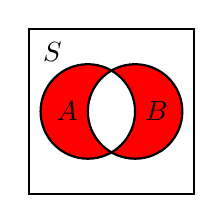
\begin{tikzpicture}[thick, scale=0.3]
  \draw (-3.5, -3.5) rectangle (3.5, 3.5);
\fill[red] (0,0 |- 60:2cm) arc [start angle=60, end angle = 300, radius = 2cm]
                           arc [start angle=240, end angle = 120, radius = 2cm];
\fill[red] (0,0 |- 60:2cm) arc [start angle=120, end angle = -120, radius = 2cm]
                           arc [start angle=-60, end angle = 60, radius = 2cm];
  \draw (-1,0) circle [radius=2cm]
               (1,0) circle [radius=2cm];
  \draw (-1,0) node[left] {$A$};
  \draw (1,0) node[right] {$B$};
  \draw (-2.5,2.5) node {$S$};
\end{tikzpicture}
  \end{minipage}
\begin{Ex}
  \begin{itemize}
  \item $\{1,2\} \bigtriangleup \{2,3\} = \{1,3\}$
  \end{itemize}
\end{Ex}
\end{frame}

\begin{frame}
    \begin{Def}  
    以集合为元素的集合称为集族。如果$I$为任意一个集合,对$I$中每个元素$\alpha$都有一个唯一的集合与之对应,这个集合记为$A_{\alpha}$,那么所有这些$A_{\alpha}$形成的集族可以用$\{A_{\alpha}\}_{\alpha \in I}$表示,其中$I$称为标号集。
  \end{Def}
  \begin{Ex}
    \begin{itemize}
    \item 设标号集$I=\{1,2,3\}$,那么$\{A_{\alpha}\}_{\alpha \in I}=\{A_1,A_2,A_3\}$
    \item 设标号集$I=Z^+$,那么$\{A_{\alpha}\}_{\alpha \in I}=\{A_1,A_2,A_3,\cdots\}$
    \end{itemize}
  \end{Ex}
\end{frame}
\begin{frame}
  \begin{Def}
    集族$\{A_{\alpha}\}_{\alpha \in I}$中所有集合的并集$\bigcup_{\alpha \in I}A_{\alpha}$定义为
\[ \bigcup_{\alpha \in I}A_{\alpha} = \{x|\exists \alpha \in I x \in A_{\alpha}\}\]
    集族$\{A_{\alpha}\}_{\alpha \in I}$中所有集合的交集$\bigcap_{\alpha \in I}A_{\alpha}$定义为
\[ \bigcap_{\alpha \in I}A_{\alpha} = \{x|\forall \alpha \in I x \in A_{\alpha}\}\]
\end{Def}
  \begin{Ex}
    \begin{itemize}
    \item 设标号集$I=\{1,2,3\}$,那么$\bigcup_{\alpha \in I}A_{\alpha}=A_1\cup A_2 \cup A_3$
    \item 设标号集$I=Z^+$,那么$\bigcup_{\alpha \in I}A_{\alpha}=\{x|\exists \alpha \in Z^+ \text{使得} x \in A_{\alpha}\}$,并可记为$\bigcup_{i=1}^{\infty}A_i$
    \end{itemize}
  \end{Ex}
\end{frame}
\begin{frame}
    \begin{Def}
    两个对象按照一定的顺序排列构成的整体称为一个{\bfseries 有序对}。如果第一个对象为$a$ ,第二个对象为$b$ ,则该有序对记为$(a,b)$。$(a,b)=(c,d)$当且仅当$a=c$并且$b=d$。
  \end{Def}
  \begin{Def}\justifying\let\raggedright\justifying
    设$A$与$B$为任意两个集合,则称集合 $\{(a,b)|a\in A \land b \in B\}$为$A$与$B$的{\bfseries 笛卡尔乘积},记为$A \times B$。
即
\begin{equation*}
  A \times B = \{(a,b)|a \in A \land b \in B\}
\end{equation*}
  \end{Def}
  \begin{Ex}
    如果$X=\{1,2\}$,$Y=\{3,4,5\}$,那么$X \times Y = ?$, $Y \times X = ?$
    \begin{equation*}
      \begin{split}
       X \times Y &= \{ (1,3), (1,4), (1,5), (2,3), (2,4), (2, 5) \}\\
       Y \times X &= \{(3,1), (3,2), (4,1), (4,2), (5,1), (5,2)\}
      \end{split}
    \end{equation*}
  \end{Ex}
\end{frame}
\begin{frame}
    \begin{Def}
    $n$个对象按照一定的顺序排列构成的整体称为一个{\bfseries $n$元组}。如果第一个对象为$a_1$,第二个对象为$a_2$,$\ldots$,第$n$个对象为$a_n$,则该$n$元组记为$(a_1,a_2, \ldots, a_n)$。
 $(a_1,a_2, \ldots, a_n)=(b_1,b_2, \ldots, b_n)$当且仅当$a_1=b_1$,$a_2=b_2$,$\ldots$,$a_n=b_n$。
  \end{Def}
  \begin{Def}
    设$A_1$, $A_2$,$\ldots$,$A_n$为任意$n$个集合,则称集合 \[\{(a_1,a_2, \ldots, a_n)|a_i\in A_i, i = 1,2,\ldots, n\}\] 为$A_1, A_2, \ldots, A_n$ 的{\bfseries 笛卡尔乘积},记为$A_1 \times A_2 \times \cdots \times A_n$, 简记为$\prod_{i=1}^nA_i$。即
\begin{equation*}
  A_1 \times A_2 \times \cdots \times A_n = \prod_{i=1}^nA_i = \{(a_1,a_2, \ldots, a_n)|a_i \in A_i, i = 1, 2, \cdots, n\}
\end{equation*}

当$A_1=A_2=\cdots=A_n=A$时,$A_1 \times A_2\times \cdots \times A_n$简记为$A^n$,例如$A^2=A\times A$,$A^3=A\times A\times A$。
我们以前熟知的二维空间$R^2$即为$R\times R$,三维空间$R^3$即为$R\times R\times R$。
\end{Def}
\end{frame}
\begin{frame}
    \begin{Ex}
    如果$X=\{a_1,b_1\}$,$Y=\{a_2,b_2\}$,$Z=\{a_3,b_3\}$ 那么 $X \times Y \times Z = ?$
    \begin{equation*}
      \begin{split}
       X \times Y \times Z =& \{ (a_1,a_2, a_3), (a_1,a_2, b_3), (a_1, b_2, a_3), (a_1,b_2, b_3), \\
&(b_1, a_2, a_3), (b_1, a_2, b_3), (b_1, b_2, a_3), (b_1, b_2, b_3) \}\\
      \end{split}
    \end{equation*}
  \end{Ex}
\end{frame}
\begin{frame}
    \begin{Def}
    设$X$和$Y$为两个非空集合。一个从$X$到$Y$的{\bfseries 映射}$f$为一个法则,根据$f$,对$X$中的每个元素$x$都有$Y$中唯一确定的元素$y$与之对应。
    从$X$到$Y$的映射$f$常记为$f:X\to Y$。
  \end{Def}
  \begin{Ex}
    设集合$X=\{-1,0,1\}$,集合$Y=\{0,1,2\}$,$\forall x \in X, f(x)=x^2$,即$f(-1)=1,f(0)=0,f(1)=1$,则$f$为从集合$X$到集合$Y$的映射。
  \end{Ex}
\end{frame}
\begin{frame}
    \begin{Def}
    设$X$和$Y$为两个非空集合。一个从$X$到$Y$的{\bfseries 映射}为一个满足以下两个条件的$X\times Y$的子集$f$:
    \begin{enumerate}
    \item 对$X$的每一个元素$x$,存在一个$y\in Y$,使得$(x,y) \in f$;
    \item 若$(x,y)\in f$,$(x,y')\in f$,则$y=y'$。
    \end{enumerate}
    $(x,y)\in f$记为$y=f(x)$。
  \end{Def}
  \begin{Ex}\justifying\let\raggedright\justifying
    设集合$X=\{-1,0,1\}$,集合$Y=\{0,1,2\}$,$f=\{(-1,1),(0,0),(1,1)\}$,则$f$为从集合$X$到集合$Y$的映射。
  \end{Ex}
\end{frame}
\begin{frame}
    \begin{Def}
    设$f$为从集合$X$到集合$Y$的映射,$f:X\to Y$, 如果$y = f(x)$,则称$y$为$x$在$f$下的{\bfseries 象},称$x$为$y$的{\bfseries 原象}。$X$称为$f$的{\bfseries 定义域};集合$\{f(x) | x \in X\}$称为$f$的{\bfseries 值域},记为$Im(f)$。
  \end{Def}
\end{frame}
\begin{frame}
    \begin{Def}
    设$f:X\to Y$,如果$\forall x_1, x_2 \in X$, 只要$x_1 \neq x_2$,  就 有 $f(x_1) \neq f(x_2)$,   则称$f$为从$X$到$Y$的{\bfseries 单射}。
  \end{Def}
  \begin{Def}
    设$f:X\to Y$, 如果$\forall y \in Y$, $\exists x \in X$使得 $f(x) = y$, 则称$f$为从$X$到$Y$的{\bfseries 满射}。
  \end{Def}
  \begin{Def}
    设$f:X\to Y$,如果$f$既是单射又是满射,则称$f$为从$X$到$Y$的{\bfseries 双射},或者称$f$为从$X$到$Y$的一一对应。
  \end{Def}
\end{frame}
\begin{frame}
    \begin{Def}
    设$f:X\to Y$,$A \subseteq X$,$A$在$f$下的{\bfseries 象}定义为\[f(A)=\{f(x)|x\in A\}\]
  \end{Def}
  \begin{Ex}
    设$f:\{-1,0,1\}\to \{-1,0,1\}$,$f(x)=x^2$,则$f(\{-1,0\})=\{0,1\}$
  \end{Ex}
\end{frame}
\begin{frame}
    \begin{Def}
    设$f:X\to Y$,$B \subseteq Y$,$B$在$f$下的{\bfseries 原象}定义为\[f^{-1}(B)=\{x\in X|f(x)\in B\}\]
  \end{Def}
  \begin{Ex}
    设$f:\{-1,0,1\}\to \{-1,0,1\}$,$f(x)=x^2$,则$f^{-1}(\{-1,0\})=\{0\}$
  \end{Ex}
\end{frame}
\begin{frame}
   \begin{Def}
    设$f:X\to Y$,$g:Y\to Z$为映射,映射$f$与$g$的{\bfseries 合成}$g\circ f:X\to Z$定义为\[(g\circ f)(x) = g(f(x))\]
  \end{Def}
\end{frame}
\begin{frame}
   \begin{Def}
     设$f:X\to Y$为双射,$f$的{\bfseries 逆映射}$f^{-1}:Y\to X$定义为:对任意的$y\in Y$,存在唯一的$x$使得$f(x)=y$,则$f^{-1}(y)=x$。
   \end{Def}

   \begin{Def}\label{inverse1}
          设$f:X\to Y$为一个双射, 则$g:Y\to X, g=\{(y,x)|(x,y)\in f\}$称为$f$的{\bfseries 逆映射},记为$g=f^{-1}$。
   \end{Def}
   \begin{Ex}
     设集合$X=\{1,2,3\}$,$Y=\{4,5,6\}$,$f=\{(1,4),(2,5),(3,6)\}$为从$X$到$Y$的双射,则$f^{-1}=\{(4,1),(5,2),(6,3)\}$。
   \end{Ex}
 \end{frame}
 \begin{frame}
       \begin{Def}\label{inverse2}
     设$f:X\to Y$为一个映射。如果存在一个映射$g:Y\to X$使得\[f\circ g = I_{Y} \text{且} g\circ f = I_{X},\]则称映射$f$为{\bfseries 可逆}的,而$g$称为$f$的{\bfseries 逆映射}。
   \end{Def}
      \begin{Ex}
     设集合$X=\{1,2,3\}$,$Y=\{4,5,6\}$,$f=\{(1,4),(2,5),(3,6)\}$为从$X$到$Y$的双射,$g=\{(4,1),(5,2),(6,3)\}$,由于$f\circ g = I_{Y}$且$ g\circ f = I_{X}$,$f^{-1}=g$。
   \end{Ex}
 \end{frame}
 \begin{frame}
   \begin{Def}
    设$A$与$B$为两个集合。一个从$A\times B$到$\{T,F\}$的映射$R$,称为从$A$到$B$的一个{\bfseries 二元关系}。
    $\forall (a,b) \in A \times B$,如果$(a,b)$在$R$下的象为$T$,则称$a$与$b$符合关系$R$,记为$aRb$;
    如果(a,b)在$R$下的象为$F$,则称$a$与$b$不符合关系$R$,记为$aR\!\!\! / b$。如
    果$A=B$,则称$R$为$A$上的二元关系。
  \end{Def}
  \begin{Ex}
  设集合$X=\{1,2\}$,则$2^X$上的二元关系$\subseteq$可以定义为一个从$2^X\times
  2^X$到$\{T,F\}$的映射,

  $\subseteq(\{\phi\},\{\phi\})=T,\subseteq(\{\phi\},\{1\})=T,\subseteq(\{\phi\},\{2\})=T,\subseteq(\{\phi\},\{1,2\})=T,$

    $\subseteq(\{1\},\{\phi\})=F,\subseteq(\{1\},\{1\})=T,\subseteq(\{1\},\{2\})=F,\subseteq(\{1\},\{1,2\})=T,$

      $\subseteq(\{2\},\{\phi\})=F,\subseteq(\{2\},\{1\})=F,\subseteq(\{2\},\{2\})=T,\subseteq(\{2\},\{1,2\})=T,$

        $\subseteq(\{1,2\},\{\phi\})=F,\subseteq(\{1,2\},\{1\})=F,\subseteq(\{1,2\},\{2\})=F,\subseteq(\{1,2\},\{1,2\})=T$
      \end{Ex}
    \end{frame}
    \begin{frame}      
      \begin{Def}
    设$A$与$B$为两个集合。$A\times B$的任一子集$R$称为从$A$到$B$的一个{\bfseries 二元关系}。如果$(a,b)\in R$,则称$a$与$b$符合关系$R$,记为$aRb$;如果$(a,b) \notin R$,则称$a$与$b$不符合关系$R$,并记为$aR\!\!\! / b$。
    如果$A=B$,则称$R$为$A$上的二元关系。
  \end{Def}
    \begin{Ex}
  设集合$X=\{1,2\}$,则$2^X$上的二元关系$\subseteq$可以定义为$2^X\times
  2^X$的一个子集,

  \begin{equation*}
    \begin{split}
 \subseteq =& \{
 (\{\phi\},\{\phi\}),(\{\phi\},\{1\}),(\{\phi\},\{2\}),(\{\phi\},\{1,2\}),\\
 &(\{1\},\{1\}),(\{1\},\{1,2\}),(\{2\},\{2\}),(\{2\},\{1,2\}),\\
 &(\{1,2\},\{1,2\})
\}
    \end{split}
  \end{equation*}
\end{Ex}
\end{frame}
\begin{frame}
    \begin{Def}
    集合$X$上的二元关系$R$称为{\bfseries 等价关系},如果$R$同时满足以下三个性质:
    \begin{enumerate}
    \item $R$为自反的,即对$X$中的任意元素$x$,$xRx$;
    \item $R$为对称的,即对$X$中的任意元素$x$,$y$,如果$xRy$,则$yRx$;
    \item $R$为传递的,即对$X$中的任意元素$x$,$y$,$z$,如果$xRy$且$yRz$,则$xRz$。
    \end{enumerate}
  \end{Def}
  \begin{Ex}
    \begin{itemize}
    \item     整数集$\mathbb{Z}$上的模$n$同余关系为$\mathbb{Z}$上的等价关系。
    \item 设集合
    $X=\{1,2,3,4,5,6 \}$上的关系$R$定义如下:
    \begin{align*}
      R=&\{(1,1),(1,3),(1,5),(2,2),(2,4),(3,1),(3,3),(3,5),(4,2),\\
      &(4,4),(5,1),(5,3),(5,5),(6,6)\},
    \end{align*}
      则$R$为$X$上的等价关系。
    \end{itemize}
  \end{Ex}
\end{frame}

\begin{frame}
     \begin{Def}
    设$X$为集合, $X$的一些非空子集形成的集族$\mathscr{A}$称为$X$的一个{\bfseries 划分},如果$\mathscr{A}$具有性质
    \begin{enumerate}
    \item $\forall A, B \in \mathscr{A}$,如果$A \neq B$,则$A \cap B = \phi$;
      \item $\bigcup_{A \in \mathscr{A}} = X$
    \end{enumerate}
  \end{Def}

  \begin{Ex}
    \begin{itemize}
    \item     集合
    \begin{equation*}
      \begin{split}
      \{&\{\cdots,-8,-4,0,4,8,\cdots\},\\
      &\{\cdots,-7,-3,1,5,9,\cdots\},\\
      &\{\cdots,-6,-2,2,6,10,\cdots\},\\
      &\{\cdots,-5,-1,3,7,11,\cdots\}\}
    \end{split}
  \end{equation*}
  构成了整数集$\mathbb{Z}$的一个划分。
\item     集合$\{\{1,3,5\},\{2,4\},\{6\}\}$构成了集合$X=\{1,2,3,4,5,6\}$的一个划分。
\end{itemize}
\end{Ex}
\end{frame}
\begin{frame}
    \begin{Def}
    集合$X$上的二元关系$R$称为{\bfseries 偏序关系},如果$R$同时满足以下三个性质:
    \begin{enumerate}
    \item $R$为自反的,即对$X$中的任意元素$x$,$xRx$;
    \item $R$为反对称的,即对$X$中的任意元素$x$,$y$,如果$xRy$且$yRx$,则$x=y$;
    \item $R$为传递的,即对$X$中的任意元素$x$,$y$,$z$,如果$xRy$且$yRz$,则$xRz$。
    \end{enumerate}
  \end{Def}
    \begin{Def}
    设$\leq$为集合$X$上的一个偏序关系,则称二元组$(X,\leq)$为一个{\bfseries 偏序集}。
  \end{Def}

  \begin{Ex}
    \begin{itemize}
    \item  实数集$\mathbb{R}$上通常的“小于等于”关系$\leq$为一个偏序关系,所以$(\mathbb{R},\leq)$为一个偏序集。
    \item  设$S$为一个集合,$S$的子集间的包含关系$\subseteq$为$2^S$上的一个偏序关系,所以$(2^{\mathbb{S}},\subseteq)$为一个偏序集。
    \end{itemize}
  \end{Ex}
\end{frame}

\begin{frame}
    \begin{Def}
    设$(X,\leq)$为一个偏序集,$A\subseteq X$。如果存在一个元素$s\in A$使得$\forall x \in A$有$x \leq s$,则称$s$为$A$的{\bfseries 最大元素};如果存在一个元素$t\in A$使得$\forall x \in A$有$t \leq x$,则称$t$为$A$的{\bfseries 最小元素}。
  \end{Def}
\end{frame}

\begin{frame}
    我们用$x<y$表示$x\leq y$且$x\neq y$。
    \begin{Def}
    设$(X,\leq)$为一个偏序集,$A\subseteq X$。如果存在一个元素$s\in A$,在$A$中没
    有元素$x$使得$s < x$,则称$s$为$A$的{\bfseries 极大元素};如果存在一个元素$t\in A$,在$A$中没有元素$x$使得$x < t$,则称$t$为$A$的{\bfseries 极小元素}。
  \end{Def}
\end{frame}

\begin{frame}
      \begin{Def}
    设$(X,\leq)$为一个偏序集,$A\subseteq X$。如果存在一个元素$s\in X$使得$\forall x \in A$有$x \leq s$,则称$s$为$A$的一个{\bfseries 上界};如果存在一个元素$t\in X$使得$\forall x \in A$有$t \leq x$,则称$t$为$A$的一个{\bfseries 下界}。
  \end{Def}
\end{frame}

\begin{frame}
      \begin{Def}
      设$(X,\leq)$为一个偏序集,$A\subseteq X$。如果$A$有上界且$A$的一切上界之集有最小元素,则这个最小上界称为$A$的{\bfseries 上确界},记为$\sup A$;如果$A$有下界且$A$的一切下界之集有最大元素,则这个最大下界称为$A$的{\bfseries 下确界},记为$\inf A$。
  \end{Def}
\end{frame}

\begin{frame}
    \begin{Def}
    如果从集合$X$到集合$Y$存在一个双射,则称$X$与$Y${\bfseries 对等},记为$X \sim Y$。
  \end{Def}

  \begin{Def}
设$A$为一个集合,如果$A=\Phi$,其{\bfseries 基数}定义为$0$;如果$A \neq \Phi$且存在一个自然数$n$使得$A$与集合$\{1,2,\ldots, n\}$之间存在一个一一对应,则定义$A$的{\bfseries 基数}为$n$。$A$的基数记为$|A|$。如果$|A|$为0或某个自然数$n$,则称$A$为有穷集;如果A不是有穷集,则称$A$为无穷集。   
  \end{Def}

    \begin{Def}
    如果从自然数集$\mathbb{N}$到集合$X$存在一个一一对应$f:\mathbb{N}\to X$,则称
    集合$X$为{\bfseries 可数无穷集合},简称{\bfseries 可数集}或{\bfseries 可列集}。如果$X$不是可数集且$X$不是有穷集合,则称$X$为{\bfseries 不可数无穷集合},简称{\bfseries 不可数集}。
  \end{Def}
\end{frame}
\begin{frame}
    \begin{Def}
    凡与集合$[0,1]$存在一个一一对应的集合称为具有“连续统的势”的集合,简称连续统。
  \end{Def}
\end{frame}
\begin{frame}
      \begin{Def}
    集合$A$的{\bfseries 基数}为一个符号,凡与$A$对等的集合都赋以同一个记号。集合$A$的基数记为$|A|$。
  \end{Def}
  \begin{Def}
    所有与集合$A$对等的集合构成的集族称为$A$的{\bfseries 基数}。
  \end{Def}
  \begin{Def}
    集合$A$的基数与集合$B$的基数称为是相等的,当且仅当$A \sim B$。
  \end{Def}
\end{frame}
\begin{frame}
    \begin{Def}
    设$\alpha$,$\beta$为任意两个基数,$A$,$B$为分别以$\alpha$,$\beta$为其基数的
    集合。如果$A$与$B$的一个真子集对等,但$A$却不能与$B$对等,则称基数$\alpha$小于基数$\beta$,记为$\alpha < \beta$。
  \end{Def}
  显然,
  $\alpha \leq \beta$当且仅当存在单射$f:A \to B$。

  $\alpha < \beta$当且仅当存在单射$f:A \to B$且不存在$A$到$B$的双射。
\end{frame}

\begin{frame}
  设$V$为一个集合,$V$的一切二元子集之集合记为$\mathcal{P}_2(V)$,即
\begin{equation*}
  \mathcal{P}_2(V) = \{A|A \subseteq V \text{且} |A| = 2\}\text{。}
\end{equation*}
\begin{Def}
  设$V$为一个非空有限集合,$E \subseteq \mathcal{P}_2(V)$,二元组$G = (V, E)$称为一个无向图。$V$中的元素称为无向图$G$的顶点,$V$为顶点集;$E$中的元素称为无向图$G$的边,$E$为边集。无向图简称图。如果$|V|=p$,$|E|=q$,则称$G$为一个$(p,q)$图,即$G$是一个具有$p$个顶点$q$条边的图。
\end{Def}
      \centering
    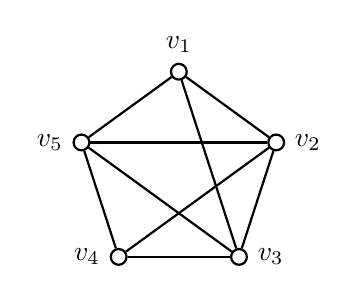
\begin{tikzpicture}[auto,
    specification/.style ={circle, draw, thick, inner sep = 0pt, minimum size=2mm}]
   \node[specification] (A)  [label=0:$v_2$] at (18:1.3cm)  {};
   \node[specification] (B)  [label=90:$v_1$] at (90:1.3cm)  {};
   \node[specification] (C)  [label=180:$v_5$] at (162:1.3cm)  {};
   \node[specification] (D) [label=180:$v_4$] at (234:1.3cm)  {};
   \node[specification] (E)  [label=0:$v_3$] at (306:1.3cm)  {};      
   
   
   \draw[thick] (A) to  (B);
   \draw[thick] (B) to  (C);
   \draw[thick] (C) to  (D);
   \draw[thick] (D) to  (E);
   \draw[thick] (E) to  (A);
   \draw[thick] (A) to  (C);
   \draw[thick] (B) to  (E);
   \draw[thick] (C) to  (E);
   \draw[thick] (D) to  (A);
 \end{tikzpicture}
\end{frame}
\begin{frame}
    \begin{Def}
    设$G=(V,E)$为一个图,图$H=(V_1,E_1)$称为$G$的一个{\bfseries 子图},当且仅当$V_1$为$V$的
    非空子集且$E_1$为$E$的子集。如果$H \neq G$,则称$H$为$G$的{\bfseries 真子图}。
  \end{Def}
  \begin{Def}
    设图$G$的子图$H$具有某种性质,若$G$中不存在与$H$不同的具有此性质且包含$H$的子图,则称$H$是具有此性质的{\bfseries 极大子图}。
  \end{Def}
    \begin{Def}
    设$S$为图$G=(V,E)$的顶点集$V$的非空子集,则$G$的以$S$为顶点集的极大子图称为由$S$导出的子图,记为$\langle S \rangle$。
形式的,
\begin{equation*}
  \langle S \rangle=(S, \mathcal{P}_2(S) \cap E)
\end{equation*}
  \end{Def}
\end{frame}
\begin{frame}
    \begin{Def}
    设$G=(V,E)$为一个图。$G$的一条{\bfseries 通道}为$G$的顶点和边的一个交错序列
    \[v_0,x_1,v_1,x_2,v_2,x_3,\ldots,v_{n-1},x_n,v_n\]
    其中$x_i=\{v_{i-1},v_i\},i=1,2,\ldots,n$。$n$称为该通道的长。这样的通道常称为$v_0-v_n$通道,并简记为$v_0v_1v_2\ldots   v_n$。如果通道的长大于等于$1$且$v_0=v_n$,则称此通道为{\bfseries 闭通道}。
  \end{Def}
  \begin{Def}
   如果图中一条通道上的各边互不相同,则称此通道为图的{\bfseries 迹}。如果一条闭通道上的各边互不相同,则称此闭通道为{\bfseries 闭迹}。
  \end{Def}
  \begin{Def}
    如果一条迹上的各顶点互不相同,则称此迹为路。如果闭迹上除终点外各顶点互不相同,则称此闭迹为{\bfseries 圈},或{\bfseries 回路}。
  \end{Def}
\end{frame}
\begin{frame}
     \begin{Def}
    图$G$的极大连通子图称为$G$的一个支。
  \end{Def}
  \vspace{1cm}
  \centering
  \begin{minipage}{0.33\linewidth}
    \centering
    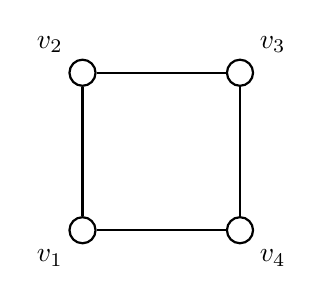
\begin{tikzpicture}[auto,
    specification/.style ={circle, draw, thick}]
   \node[specification] (A) [label=-135:$v_1$] at (0,0)  {};
   \node[specification] (B) [label=135:$v_2$] at (0,2)  {};
   \node[specification] (C) [label=45:$v_3$] at (2,2)  {};
   \node[specification] (D) [label=-45:$v_4$] at (2,0)  {};
   \draw[thick] (A) to  (B);
   \draw[thick] (B) to  (C);
   \draw[thick] (C) to  (D);
   \draw[thick] (D) to  (A);
 \end{tikzpicture}
\end{minipage}\hfill
\begin{minipage}{0.33\linewidth}
  \centering
  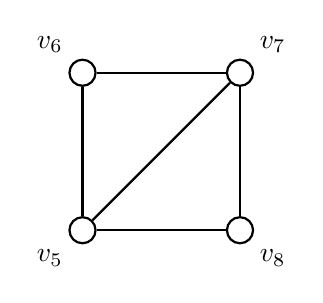
\begin{tikzpicture}[auto,
    specification/.style ={circle, draw, thick}]
   \node[specification] (E) [label=-135:$v_5$] at (0,0)  {};
   \node[specification] (F) [label=135:$v_6$] at (0,2)  {};
   \node[specification] (G) [label=45:$v_7$] at (2,2)  {};
   \node[specification] (H) [label=-45:$v_8$] at (2,0)  {};
   \draw[thick] (E) to  (F);
   \draw[thick] (F) to  (G);
   \draw[thick] (G) to  (H);
   \draw[thick] (H) to  (E);
   \draw[thick] (E) to  (G);
 \end{tikzpicture}  
\end{minipage}\hfill
\begin{minipage}{0.33\linewidth}
  \centering
  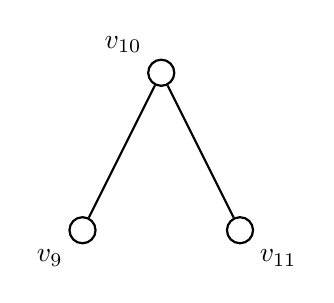
\begin{tikzpicture}[auto,
    specification/.style ={circle, draw, thick}]
   \node[specification] (I) [label=-135:$v_9$] at (0,0)  {};
   \node[specification] (J) [label=135:$v_{10}$] at (1,2)  {};
   \node[specification] (K) [label=-45:$v_{11}$] at (2,0)  {};
   \draw[thick] (I) to  (J);
   \draw[thick] (J) to  (K);
 \end{tikzpicture}
\end{minipage}
\vspace*{2cm}
$G$
\end{frame}
\begin{frame}
    \begin{Thm}
    设$G=(V,E)$是一个图。在$V$上定义二元关系$\cong$如下:\[\forall u, v \in V, u
      \cong v\text{当且仅当}u\text{与}v\text{间有一条路,}\]则$\cong$为$V$上的等价关系,$G$的支就是关于$\cong$的每个等价类的导出子图。
  \end{Thm}
\end{frame}
\begin{frame}
  \begin{Def}
  设$G=(V,E)$为一个图,$V=\{v_1,v_2,\ldots,v_p\}$。$p\times p$矩阵$A=(a_{ij})$称为$G$的邻接矩阵,其中
  \[a_{ij}=\begin{cases}
      1, \text{如果}\{v_i,v_j\}\in E\\
      0, \text{如果}\{v_i,v_j\}\notin E\\
    \end{cases}
  \]
\end{Def}
 \begin{Def}
   设$G=(V,E)$为一个有$p$个顶点$q$条边的图,$V=\{v_1,v_2,\ldots, v_p\}$,$E=\{e_1,e_2,\ldots,e_q\}$,$p\times q$矩阵$M=(m_{ij})$称为$G$的关联矩阵,其中
  \[m_{ij}=\begin{cases}
      1, \text{如果}v_i\text{与边}e_j\text{相关联}\\
      0, \text{如果}v_i\text{不与边}e_j\text{相关联}
    \end{cases}
  \]
 \end{Def}

\end{frame}
\begin{frame}
    \begin{Def}
    设$V$为一个有穷非空集合,$A \subseteq V\times V \setminus \{(v,v)|v \in V\}$,二元组$D=(V,A)$称为一个{\bfseries 有向图}。$V$称为有向图$D$的{\bfseries 顶点集},$V$中的元素称为$D$的{\bfseries 顶点}。
    $A$称为$D$的{\bfseries 弧集}或{\bfseries 有向边集},$A$中的元素称为$D$的{\bfseries 弧}或{\bfseries 有向边}。如果$x = (u,v) \in A$,则$u$称为弧$x$的{\bfseries 起点},$v$称为弧$x$的{\bfseries 终点}。
  \end{Def}
    \centering
  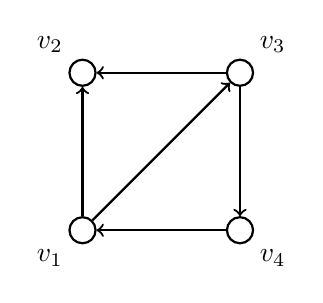
\begin{tikzpicture}[auto,
    specification/.style ={circle, draw, thick}]
   \node[specification] (A) [label=-135:$v_1$] at (0,0)  {};
   \node[specification] (B) [label=135:$v_2$] at (0,2)  {};
   \node[specification] (C) [label=45:$v_3$] at (2,2)  {};
   \node[specification] (D) [label=-45:$v_4$] at (2,0)  {};
   \draw[thick, ->] (A) to  (B);
   \draw[thick, ->] (C) to  (B);
   \draw[thick, ->] (C) to  (D);
   \draw[thick, ->] (D) to  (A);
   \draw[thick, ->] (A) to  (C);
\end{tikzpicture}
\end{frame}
\begin{frame}
    \begin{Def}
    设$D=(V,A)$为一个有向图,有向图$H=(V_1,A_1)$称为$D$的一个{\bfseries 子图},当且仅当$V_1$为$V$的
    非空子集且$A_1$为$A$的子集。如果$H \neq D$,则称$H$为$D$的{\bfseries 真子图}。
  \end{Def}
  
\end{frame}
\begin{frame}
    \begin{Def}
    设$D=(V,A)$为一个有向图。$D$的一条{\bfseries 有向通道}为$D$的顶点和弧的一个交错序列
    \[v_0,x_1,v_1,x_2,v_2,\cdots,v_{n-1},x_n,v_n \]
    其中$x_i = (v_{i-1},v_i)$, $i=1,2,\cdots, n$。$n$称为该有向通道的长。 这样的有向通道常称为$v_0-v_n$有向通道,并简记为$v_0v_1v_2\ldots v_n$。如果有向通道的长大于等于$1$且$v_0=v_n$,则称此有向通道为{\bfseries 闭有向通道}。
  \end{Def}
    \begin{Def}
如果有向图中一条有向通道的各弧互不相同,则称此有向通道为有向图的{\bfseries 有向迹}。如果一条闭有向通道上的各弧互不相同,则称此闭有向通道为{\bfseries 闭有向迹}。   
  \end{Def}
  \begin{Def}
如果一条有向迹上的各顶点互不相同,则称此有向迹为{\bfseries 有向路}。如果闭有向迹上除终点外各顶点互不相同,则称此闭有向迹为{\bfseries 有向圈},或{\bfseries 有向回路}。
  \end{Def}
\end{frame}
\begin{frame}
     \begin{Def}
    设$D=(V,A)$为一个有向图,$u$和$v$为$D$的顶点。如果在$D$中有一条从$u$到$v$的
    有向路,则称从$u$能达到$v$,或者$v$是从$u${\bfseries 可达}的。
  \end{Def}
  \begin{Def}
   有向图$D$称为是{\bfseries 强连通}的,如果对$D$的任意两个不同的顶点$u$和$v$,$u$和$v$是互达的(即从$u$可以达到$v$并且从$v$可以达到$u$)。 
  \end{Def}
\end{frame}
\begin{frame}
     \begin{Def}
   有向图$D$的极大强连通子图称为$D$的一个{\bfseries 强支}。 
 \end{Def}
      \begin{Thm}
      设$D=(V,A)$为一个有向图。在$V$上定义二元关系$\cong$如下:\[\forall u, v \in V, u \cong v\text{当且仅当}u\text{与}v\text{互达}\]则$\cong$为$V$上的等价关系,$D$的强支就是关于$\cong$的每个等价类的导出子图。
    \end{Thm}
       \begin{Def}
   有向图$D=(V,A)$称为{\bfseries 单向连通}的,如果对$D$的任意两个不同的顶点$u$和$v$,或从$u$可达到$v$,或从$v$可达到$u$。 
 \end{Def}
    \begin{Def}
   设$D=(V,A)$为一个有向图,如果抹去$D$中所有弧的方向之后所得到的无向图是连通的,则称$D$为{\bfseries 弱连通}的,简称{\bfseries 连通}的。 
  \end{Def}
\end{frame}
\begin{frame}
   \begin{Def}
   设$D=(V,A)$为一个有向图,$V=\{v_1,v_2,\ldots, v_p\}$,$p\times p$矩阵$B=(b_{ij})$称为$D$的邻接矩阵,其中
  \[b_{ij}=\begin{cases}
      1, \text{如果}(v_i,v_j)\in A\\
      0, \text{如果}(v_i,v_j)\notin A\\
    \end{cases}
  \]
 \end{Def}
 \begin{Def}
   设$D=(V,A)$为一个有$p$个顶点$q$条弧的有向图,$V=\{v_1,v_2,\ldots, v_p\}$,$A=\{x_1,x_2,\ldots,x_q\}$,$p\times q$矩阵$H=(h_{ij})$称为$D$的关联矩阵,其中
  \[h_{ij}=\begin{cases}
      1, \text{如果}v_i\text{为弧}x_j\text{的起点}\\
      -1, \text{如果}v_i\text{为弧}x_j\text{的终点}\\
      0, \text{如果}v_i\text{既不是弧}x_j\text{的起点也不是弧}x_j\text{的终点}
    \end{cases}
  \]
 \end{Def}
\end{frame}
\begin{frame}
  \begin{Def}
    连通且无圈的无向图称为无向树,简称{\bfseries树}。 一个没有圈的无向图
    称为无向森林,简称{\bfseries森林}。
  \end{Def}
\end{frame}
\begin{frame}
        具有$4$个顶点的互相不同构的所有无向图(同构的只算一个):

    \vspace{0.3cm}
  \centering
  \begin{minipage}{0.24\linewidth}
    \centering
    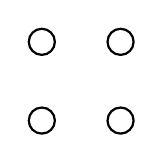
\begin{tikzpicture}[auto,
    specification/.style ={circle, draw, thick}]
   \node[specification] (A) at (0,0)  {};
   \node[specification] (B)  at (0,1)  {};
   \node[specification] (C)  at (1,1)  {};
   \node[specification] (D) at (1,0)  {};
 \end{tikzpicture}\\
 \vspace*{0.3cm}
 A
\end{minipage}\hfill 
  \begin{minipage}{0.24\linewidth}
    \centering
    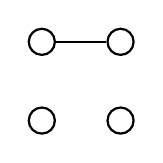
\begin{tikzpicture}[auto,
    specification/.style ={circle, draw, thick}]
   \node[specification] (A) at (0,0)  {};
   \node[specification] (B) at (0,1)  {};
   \node[specification] (C) at (1,1)  {};
   \node[specification] (D) at (1,0)  {};
   \draw[thick] (B) to  (C);
 \end{tikzpicture}\\
 \vspace*{0.3cm}
 B
\end{minipage}\hfill 
  \begin{minipage}{0.24\linewidth}
    \centering
    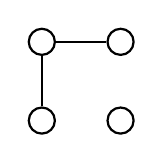
\begin{tikzpicture}[auto,
    specification/.style ={circle, draw, thick}]
   \node[specification] (A) at (0,0)  {};
   \node[specification] (B) at (0,1)  {};
   \node[specification] (C) at (1,1)  {};
   \node[specification] (D) at (1,0)  {};
   \draw[thick] (A) to  (B);
   \draw[thick] (B) to  (C);
 \end{tikzpicture}\\
 \vspace*{0.3cm}
 C
\end{minipage}\hfill 
  \begin{minipage}{0.24\linewidth}
    \centering
    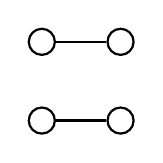
\begin{tikzpicture}[auto,
    specification/.style ={circle, draw, thick}]
   \node[specification] (A)  at (0,0)  {};
   \node[specification] (B)  at (0,1)  {};
   \node[specification] (C)  at (1,1)  {};
   \node[specification] (D) at (1,0)  {};
   \draw[thick] (B) to  (C);
   \draw[thick] (D) to  (A);
 \end{tikzpicture}\\
 \vspace*{0.3cm}
 D
\end{minipage}\hfill

\vspace*{0.5cm}
  \begin{minipage}{0.24\linewidth}
    \centering
    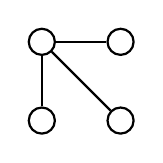
\begin{tikzpicture}[auto,
    specification/.style ={circle, draw, thick}]
   \node[specification] (A) at (0,0)  {};
   \node[specification] (B)  at (0,1)  {};
   \node[specification] (C)  at (1,1)  {};
   \node[specification] (D) at (1,0)  {};
   \draw[thick] (A) to (B);
   \draw[thick] (B) to (C);
      \draw[thick] (B) to (D);
 \end{tikzpicture}\\
 \vspace*{0.3cm}
 E
\end{minipage}\hfill
  \begin{minipage}{0.24\linewidth}
    \centering
    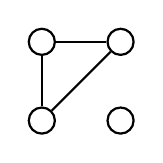
\begin{tikzpicture}[auto,
    specification/.style ={circle, draw, thick}]
   \node[specification] (A) at (0,0)  {};
   \node[specification] (B) at (0,1)  {};
   \node[specification] (C) at (1,1)  {};
   \node[specification] (D) at (1,0)  {};
   \draw[thick] (A) to  (B);
   \draw[thick] (B) to (C);
      \draw[thick] (C) to (A);
 \end{tikzpicture}\\
 \vspace*{0.3cm}
 F
\end{minipage}\hfill
  \begin{minipage}{0.24\linewidth}
    \centering
    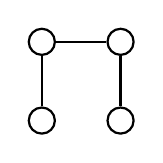
\begin{tikzpicture}[auto,
    specification/.style ={circle, draw, thick}]
   \node[specification] (A) at (0,0)  {};
   \node[specification] (B) at (0,1)  {};
   \node[specification] (C) at (1,1)  {};
   \node[specification] (D) at (1,0)  {};
   \draw[thick] (A) to  (B);
   \draw[thick] (B) to  (C);
      \draw[thick] (C) to (D);
 \end{tikzpicture}\\
 \vspace*{0.3cm}
 G
\end{minipage}\hfill 
  \begin{minipage}{0.24\linewidth}
    \centering
    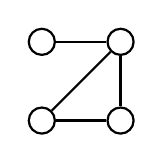
\begin{tikzpicture}[auto,
    specification/.style ={circle, draw, thick}]
   \node[specification] (A)  at (0,0)  {};
   \node[specification] (B)  at (0,1)  {};
   \node[specification] (C)  at (1,1)  {};
   \node[specification] (D) at (1,0)  {};
   \draw[thick] (A) to  (C);
   \draw[thick] (C) to  (D);
   \draw[thick] (D) to (A);
   \draw[thick] (C) to (B);
 \end{tikzpicture}\\
 \vspace*{0.3cm}
 H
\end{minipage}\hfill 

\vspace*{0.5cm}
\flushleft
  \begin{minipage}{0.24\linewidth}
    \centering
    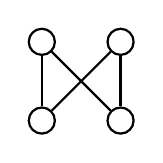
\begin{tikzpicture}[auto,
    specification/.style ={circle, draw, thick}]
   \node[specification] (A) at (0,0)  {};
   \node[specification] (B)  at (0,1)  {};
   \node[specification] (C)  at (1,1)  {};
   \node[specification] (D) at (1,0)  {};
   \draw[thick] (A) to (B);
   \draw[thick] (B) to (D);
   \draw[thick] (D) to (C);
      \draw[thick] (C) to (A);
 \end{tikzpicture}\\
 \vspace*{0.3cm}
 I
\end{minipage}
  \begin{minipage}{0.24\linewidth}
    \centering
    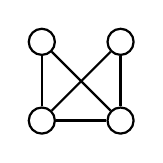
\begin{tikzpicture}[auto,
    specification/.style ={circle, draw, thick}]
   \node[specification] (A) at (0,0)  {};
   \node[specification] (B) at (0,1)  {};
   \node[specification] (C) at (1,1)  {};
   \node[specification] (D) at (1,0)  {};
   \draw[thick] (A) to  (B);
      \draw[thick] (C) to (D);
   \draw[thick] (D) to (A);
   \draw[thick] (A) to (C);
   \draw[thick] (B) to (D);
 \end{tikzpicture}\\
 \vspace*{0.3cm}
 J
\end{minipage} 
  \begin{minipage}{0.24\linewidth}
    \centering
    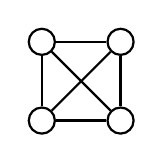
\begin{tikzpicture}[auto,
    specification/.style ={circle, draw, thick}]
   \node[specification] (A) at (0,0)  {};
   \node[specification] (B) at (0,1)  {};
   \node[specification] (C) at (1,1)  {};
   \node[specification] (D) at (1,0)  {};
   \draw[thick] (A) to  (B);
   \draw[thick] (B) to  (C);
      \draw[thick] (C) to (D);
   \draw[thick] (D) to (A);
   \draw[thick] (A) to (C);
   \draw[thick] (B) to (D);
 \end{tikzpicture}\\
 \vspace*{0.3cm}
 K
\end{minipage}

\end{frame}
\end{CJK*}
\end{document}
